\documentclass[journal,onecolumn]{IEEEtran}
\usepackage[T1]{fontenc}
\usepackage[utf8]{inputenc}
\usepackage{amsmath,amssymb}
\usepackage{graphicx}
\usepackage{booktabs}
\usepackage{multirow}
\usepackage{array}
\usepackage{tabularx}
\usepackage{xcolor}
\usepackage{url}
\usepackage[hidelinks]{hyperref}
\usepackage{tikz}
\usepackage{placeins}
\usetikzlibrary{positioning,arrows.meta,fit}
\usepackage{listings}
\lstset{basicstyle=\ttfamily\footnotesize,breaklines=true,columns=fullflexible,frame=single}
\newcolumntype{L}[1]{>{\raggedright\arraybackslash}p{#1}}

\newcommand{\ReplAbstractSentence}{All ten accuracy values of both released models were reproduced within 0.04 percentage points (vehicle mAP@0.5 78.00\% vs.\ 78.0\%); the reported parameter count of A-YOLOM(n) was not (3.64 vs.\ 4.43\,M), and Apple's MPS backend silently produced wrong metrics.}
\newcommand{\ReplDataNote}{The repository README swaps the download links of the drivable-area and lane annotations (the archive linked as \texttt{seg-drivable-10} contains the lane labels, class~11, and vice versa); we identified the archives by their class identifiers. The validation split contains 108{,}399 vehicle instances (car, bus, truck and train merged into one class, as in the original evaluation).}
\newcommand{\ReplEnvironment}{Apple M3~Pro (11-core CPU with 5 performance and 6 efficiency cores, 14-core GPU), 18\,GB unified memory, macOS~27.2.1; Python~3.10.22, PyTorch~2.2.2, torchvision~0.17.2, NumPy~1.26.4, OpenCV~4.9.0.80 and the ultralytics~8.0.105 fork contained in the repository (full list in \path{replication/requirements-lock.txt}). The official validator uses no dataloader worker processes on the CPU. One full evaluation took 51.8\,min for A-YOLOM(n) and 105.9\,min for A-YOLOM(s).}
\newcommand{\ReplDiscussion}{\textbf{Accuracy.} All ten accuracy values in Table~\ref{tab:repl} agree with the published ones within $\pm$0.04\,pp. The paper reports one decimal, so every difference is within the rounding interval ($\pm$0.05\,pp): the published evaluation of the released checkpoints is reproduced exactly, even with a newer PyTorch version (2.2.2 instead of 1.13.1) and on a CPU instead of an NVIDIA GPU. For completeness, the vehicle mAP@0.5:0.95 is 48.81\% for A-YOLOM(n) and 51.56\% for A-YOLOM(s).

\textbf{Aggregation of segmentation metrics.} The official code computes IoU and accuracy for every image and averages them. Accumulating one confusion matrix over the whole validation set gives values that are 2.1--2.8\,pp higher (Table~\ref{tab:agg}), because images with few lane or drivable-area pixels, where a few wrong pixels cost much, count as much as images with many such pixels. Neither choice is wrong, but the difference is larger than most improvements claimed in Table~\ref{tab:comparison}, and the aggregation is a detail of the evaluation code that readers cannot see unless the code is released. This gives a measured example of the comparability problem identified in RQ2.

\textbf{Parameters.} For A-YOLOM(s), the parameter count of the released checkpoint (13.61\,M before Conv+BN fusion) matches the paper. For A-YOLOM(n), both the checkpoint and the model built from the repository's configuration file have 3.64\,M parameters, not 4.43\,M as printed in the paper and README. The accuracy of this checkpoint matches the paper, so we consider the published parameter count a reporting error; its cause cannot be determined from the released material. After fusion, as used at inference, the models have 3.63\,M and 13.59\,M parameters.

\textbf{Speed.} On the M3~Pro GPU, A-YOLOM(n) reaches 37.3\,FPS at batch size~1 and 101.2\,FPS at batch size~32; A-YOLOM(s) reaches 29.5 and 53.5\,FPS. On the CPU (batch size~1) the values are 11.4 and 6.1\,FPS. Absolute values cannot be compared with the GTX~1080~Ti numbers of the paper, but the relative speed of the two models can: the paper reports a ratio n/s of 1.01 at batch size~1 and 1.79 at batch size~32; we measure 1.26 and 1.89. Both measurements time only the network forward pass, without pre-processing, NMS or mask post-processing, so they overestimate the end-to-end frame rate.

\textbf{Wrong metrics on the MPS backend.} Our first evaluation of A-YOLOM(n), with identical code, weights and data on the Apple GPU (MPS backend), gave a vehicle mAP@0.5 of 44.51\% instead of 78.00\% (Table~\ref{tab:mps}). A layer-wise comparison of the forward pass on one validation image showed no relevant difference between CPU and MPS (maximum relative difference $<3\cdot10^{-6}$). A minimal test (\path{replication/mps_inplace_view_repro.py}) shows that in PyTorch~2.2.2 an in-place \texttt{clamp\_} applied to a view of a tensor has no effect on MPS. The official post-processing and metric code use exactly this pattern: \texttt{clip\_boxes} clips predicted boxes to the image with \texttt{boxes[..., 0].clamp\_(0, w)}, and \texttt{update\_metrics\_seg} binarises masks with \texttt{mask\_list[i].clamp\_(max=1)}. We therefore attribute the discrepancy to this backend defect. No error or warning is raised, so without the published numbers as a reference this run could easily have been reported as a failed replication. Replication reports should therefore state the compute backend and, where possible, verify metrics on a second device.}
\newcommand{\ReplConclusion}{The replication confirms the published accuracy of A-YOLOM within 0.04\,pp for all ten metrics of both released models, but not the published parameter count of A-YOLOM(n), and it shows that the reported numbers also depend on how segmentation metrics are aggregated and on a correctly working compute backend}


\begin{document}

\title{Multi-Task Panoptic Driving Perception (2022--2026):\\ A Systematic Literature Review and a Replication of A-YOLOM}

\author{Priezvisko1~Meno1, Priezvisko2~Meno2, Priezvisko3~Meno3, Priezvisko4~Meno4%
\thanks{Course assignment ``Systematick\'y preh\v{l}ad literat\'ury a replik\'acia experimentu'', Umel\'a inteligencia. Replication code: see the ZIP archive accompanying this article (folder \texttt{replication/}).}}

\markboth{Assignment SOTA -- Umel\'a inteligencia}{Multi-Task Panoptic Driving Perception: Review and Replication}

\maketitle

\begin{abstract}
Camera-based \emph{panoptic driving perception} solves traffic-object detection, drivable-area segmentation and lane-line segmentation with a single network, trading a small loss of accuracy for a large gain in speed and memory. We present a systematic review of this field for 2022--2026 and a replication of one representative method. Following PRISMA~2020, we queried OpenAlex, Semantic Scholar and arXiv on 25~November~2026 with one Boolean title/abstract query, screened 100 de-duplicated records, assessed 33 full texts and included 30 studies. The included studies fall into three design families: YOLO-derived CNN encoder--decoders (18 studies), ultra-lightweight segmentation-centric networks (7) and transformer/query/prompt-based models (5). Almost all of them evaluate on the BDD100K validation split, yet results are only partially comparable. The quantity called ``lane accuracy'' denotes at least three different metrics (pixel accuracy, balanced accuracy, recall), two incompatible lane test-label protocols co-exist (reported lane IoU clusters around 25--35\% versus 56--61\%), FPS is measured on 12 different GPUs, and no included study reports variance over repeated runs. Further gaps are the absence of quantitative robustness evaluation in most studies, single-dataset evaluation and limited code availability (14 of 30). We replicated the evaluation of A-YOLOM (IEEE T-VT 2024) with the authors' code and weights on all 10{,}000 BDD100K validation images. \ReplAbstractSentence
\end{abstract}

\begin{IEEEkeywords}
Multi-task learning, panoptic driving perception, object detection, drivable-area segmentation, lane detection, BDD100K, systematic review, replication.
\end{IEEEkeywords}

%=====================================================================
\section{Introduction}
%=====================================================================
\IEEEPARstart{A}{utomated} driving requires a perception stack that recognises other traffic participants, the region in which the vehicle may drive and the lane markings that constrain its trajectory. Running a separate deep network for each of these three tasks multiplies latency, memory and energy consumption, which is a problem on embedded automotive hardware. \emph{Multi-task learning} (MTL) addresses this by sharing one encoder between several task-specific decoders~\cite{vandenhende2022mtl}. In the driving domain this idea was popularised by MultiNet~\cite{teichmann2018multinet} and DLT-Net~\cite{qian2020dltnet}. YOLOP~\cite{wu2022yolop} introduced the term \emph{panoptic driving perception} for the triple \{traffic-object detection, drivable-area segmentation, lane-line segmentation\} evaluated on BDD100K~\cite{yu2020bdd100k}. Since then, dozens of variants have been published, mostly as incremental modifications of YOLO-family detectors.

Two recent surveys cover vision-based multi-task perception broadly~\cite{review2025sensors,li2024panopticsurvey}, but neither follows a reproducible search protocol focused on the three-task BDD100K setting, nor do they examine \emph{whether the published numbers are comparable}. Our reading of the literature suggested that comparability is the central problem of the field: many papers claim state-of-the-art results that differ by fractions of a percentage point, measured with different metric definitions, label protocols and hardware. A systematic review combined with an independent replication can test this directly.

\textbf{Goal.} To systematically map camera-based multi-task driving-perception methods published in 2022--2026, to synthesise their approaches, datasets, metrics and trade-offs, to identify concrete research gaps, and to replicate one representative study. We address the following research questions:
\begin{itemize}
\item \textbf{RQ1} -- Which architectural approaches are used to solve detection, drivable-area and lane segmentation jointly, and how have they evolved?
\item \textbf{RQ2} -- Which datasets, metrics and experimental protocols are used, and to what extent are reported results comparable?
\item \textbf{RQ3} -- Which accuracy--efficiency trade-offs are reported (parameters, speed, hardware, embedded deployment)?
\item \textbf{RQ4} -- What are the main limitations and open research problems?
\item \textbf{RQ5} -- Can the published BDD100K results of A-YOLOM~\cite{wang2024ayolom} be reproduced with the released code and weights?
\end{itemize}

\textbf{Structure.} Section~\ref{sec:method} describes the review methodology, Section~\ref{sec:results} synthesises the included literature, Section~\ref{sec:discussion} discusses the findings and research gaps, Section~\ref{sec:replication} reports the replication study, Section~\ref{sec:limitations} lists limitations and Section~\ref{sec:conclusion} concludes. The use of generative AI is documented in Appendix~\ref{app:ai}.

%=====================================================================
\section{Review Methodology}\label{sec:method}
%=====================================================================
The review follows the PRISMA~2020 reporting guideline~\cite{page2021prisma}. All search outputs, screening decisions and extraction tables are included in the archive (\texttt{review/}).

\subsection{Sources and search}
The searches were run on 25~November~2026 against three open bibliographic sources with programmatic access:
(i)~\textbf{OpenAlex}~\cite{priem2022openalex}, which indexes the metadata of IEEE Xplore, ACM, Elsevier/ScienceDirect, Springer, MDPI and other publishers;
(ii)~\textbf{Semantic Scholar}~\cite{kinney2023s2} (bulk search API); and
(iii)~\textbf{arXiv} (API, title/abstract fields).
IEEE Xplore, Scopus and Web of Science were not queried directly, because we had no API access to them; their content is covered only to the extent it is indexed by OpenAlex and Semantic Scholar (see Section~\ref{sec:limitations}). The time window was 2022--2026 (publication year). The query was applied to titles and abstracts:
\begin{lstlisting}
("multi-task" OR multitask OR "panoptic driving perception")
AND ("drivable area" OR "drivable region" OR "drivable space")
AND lane
\end{lstlisting}
(the Semantic Scholar and arXiv syntaxes were adapted accordingly; the exact strings are in \texttt{review/search/fetch\_*.py}). In addition, backward citation searching in the included studies identified two frequently used baselines that the database query missed (YOLOPv2~\cite{han2022yolopv2} and TwinLiteNet~\cite{che2023twinlitenet}). Foundational works published before 2022 (BDD100K, MultiNet, DLT-Net, PRISMA, the MTL survey) are cited as background only and are not part of the synthesis.

\subsection{Eligibility criteria}
\textbf{Inclusion}: (I1)~a camera-based model that jointly solves at least two of the three tasks (traffic-object detection, drivable-area segmentation, lane-line detection/segmentation), or a study that evaluates such models; (I2)~quantitative results on BDD100K for at least two of the three tasks; (I3)~journal article, conference paper or arXiv preprint published 2022--2026 in English; (I4)~full text accessible to the authors.
\textbf{Exclusion}: (E1)~off-topic or single-task work; (E2)~secondary studies (reviews) -- used as background only; (E3)~non-English; (E4)~full text not retrievable; (E5)~no quantitative evaluation on BDD100K.

\subsection{Selection process}
Records were merged and de-duplicated by DOI and normalised title. Titles and abstracts were screened against E1--E3. Full texts were then retrieved through the open-access locations recorded by OpenAlex, arXiv or the publisher's website and assessed against I1--I4/E4--E5. The process is summarised in Fig.~\ref{fig:prisma}.

\begin{figure}[t]
\centering
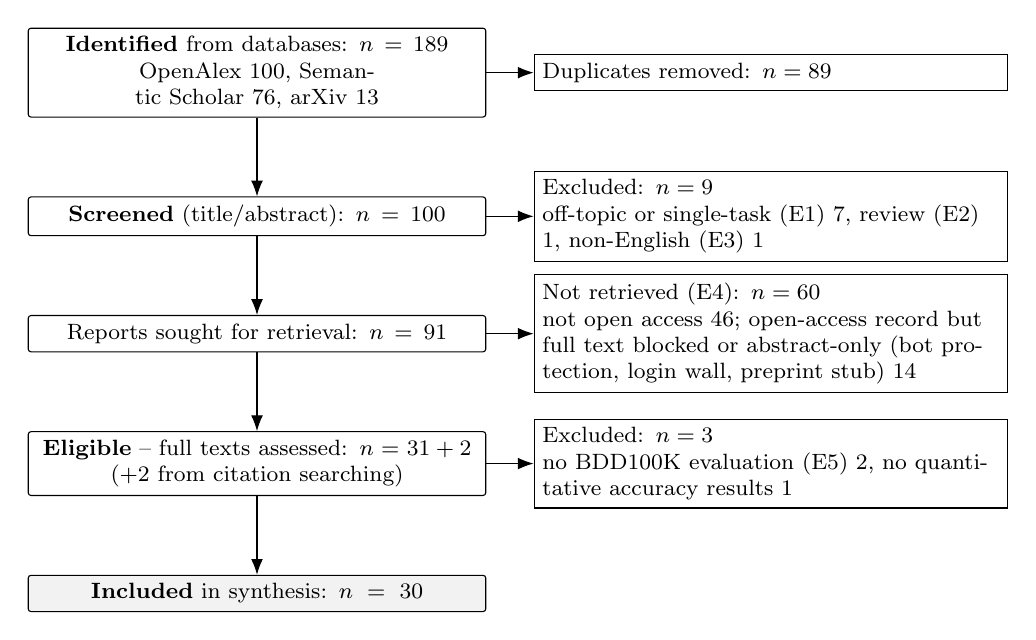
\begin{tikzpicture}[node distance=10mm and 6mm, every node/.style={font=\footnotesize}, box/.style={draw, rounded corners=1pt, align=center, text width=5.6cm, inner sep=3pt}, side/.style={draw, align=left, text width=5.8cm, inner sep=3pt}, arr/.style={-{Latex[length=2mm]}}]
\node[box] (id) {\textbf{Identified} from databases: $n=189$\\ OpenAlex 100, Semantic Scholar 76, arXiv 13};
\node[side, right=of id] (dup) {Duplicates removed: $n=89$};
\node[box, below=of id] (scr) {\textbf{Screened} (title/abstract): $n=100$};
\node[side, right=of scr] (exs) {Excluded: $n=9$\\ off-topic or single-task (E1) 7, review (E2) 1, non-English (E3) 1};
\node[box, below=of scr] (ret) {Reports sought for retrieval: $n=91$};
\node[side, right=of ret] (nret) {Not retrieved (E4): $n=60$\\ not open access 46; open-access record but full text blocked or abstract-only (bot protection, login wall, preprint stub) 14};
\node[box, below=of ret] (el) {\textbf{Eligible} -- full texts assessed: $n=31+2$\\ (+2 from citation searching)};
\node[side, right=of el] (exe) {Excluded: $n=3$\\ no BDD100K evaluation (E5) 2, no quantitative accuracy results 1};
\node[box, below=of el, fill=gray!10] (inc) {\textbf{Included} in synthesis: $n=30$};
\foreach \a/\b in {id/scr,scr/ret,ret/el,el/inc} \draw[arr] (\a) -- (\b);
\foreach \a/\b in {id/dup,scr/exs,ret/nret,el/exe} \draw[arr] (\a) -- (\b);
\end{tikzpicture}
\caption{PRISMA-style flow of the study selection (search date 25 Nov. 2026).}
\label{fig:prisma}
\end{figure}

\subsection{Data extraction and categorisation}
For each included study we extracted: publication year and venue; tasks evaluated; encoder/backbone family and detection-head type (anchor-based, anchor-free, query-based); parameter count; BDD100K results (vehicle recall and mAP@0.5, drivable-area mIoU, lane accuracy and lane IoU); the stated definition of lane accuracy; speed and the hardware it was measured on; robustness evaluation (night/weather splits, other datasets); embedded deployment; and code availability. Studies were then grouped by their dominant design principle into three families (Table~\ref{tab:qual}): \textbf{YOLO-derived} CNN encoder--decoders, \textbf{ultra-lightweight / segmentation-centric} networks, and \textbf{transformer / query / prompt-based} models. Values were copied exactly as printed in the primary source; when a value was absent we recorded ``n.r.'' (not reported).

\subsection{Tools}
Searches and de-duplication: Python~3 scripts against the OpenAlex, Semantic Scholar and arXiv APIs; bibliographic metadata: Crossref; extraction tables and figures: Python (CSV, Matplotlib); replication: PyTorch (Section~\ref{sec:replication}); writing: \LaTeX\ (IEEEtran). Full-text reading and data extraction were assisted by an LLM (Appendix~\ref{app:ai}).

%=====================================================================
\section{Results -- Literature Review}\label{sec:results}
%=====================================================================

\subsection{Overview}
The 30 included studies were published between 2022 and 2026 (Fig.~\ref{fig:years}); 22 are journal articles, 6 conference papers and 2 arXiv preprints. Every study uses BDD100K~\cite{yu2020bdd100k}, almost always with the 70k/10k train/validation split and evaluation on the 10k validation set, because the test labels are not public. Following YOLOP, the detection task is usually reduced to one merged \emph{vehicle} class (car, bus, truck, train). Table~\ref{tab:qual} summarises the design, strengths and limitations of each study and Table~\ref{tab:comparison} its reported BDD100K results.

\begin{figure}[t]
\centering
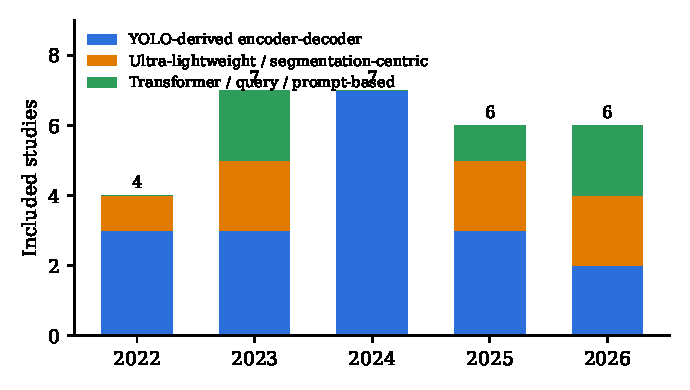
\includegraphics[width=0.62\linewidth]{figures/fig_years.pdf}
\caption{Included studies per publication year and design family (2026 covers January--November).}
\label{fig:years}
\end{figure}

\begin{table}[!htbp]
\centering
\caption{Qualitative comparison of the 30 included studies (A: YOLO-derived, B: ultra-lightweight / segmentation-centric, C: transformer / query / prompt-based). All use BDD100K; additional datasets are mentioned in the text.}
\label{tab:qual}
\scriptsize
\begin{tabularx}{\linewidth}{L{2.6cm} c c L{3.6cm} X X}
\toprule
Study & Year & Fam. & Encoder; detection head & Strengths & Limitations \\
\midrule
Multilevel-branch net~\cite{kim2022joint} & 2022 & A & n.r.; n.r. & multilevel decoder branches, +1.2\,pp DA vs.\ YOLOP & detection slightly below YOLOP; no code \\
YOLOP~\cite{wu2022yolop} & 2022 & A & CSPDarknet (YOLOv4); anchor-based & defined the task and protocol; Jetson TX2 23\,FPS & anchor-based; lane metric = recall in code \\
YOLOPv2~\cite{han2022yolopv2} & 2022 & A & E-ELAN (YOLOv7); anchor-based & strong all-round accuracy at 91\,FPS (V100) & 38.9\,M params; code not released \\
DP-YOLO~\cite{zeng2023dpyolo} & 2023 & A & YOLOv5 + inverted residual; anchor-based & 110\,FPS on T4, fewer FLOPs than YOLOP & gains $\le$0.7\,pp; no code \\
Grouped-conv/attention net~\cite{ma2023grouped} & 2023 & A & Darknet-like + grouped conv + transformer + SE; n.r. & grouped conv.\ + attention, fewer params than baseline & mAP below YOLOP; no code \\
YOLO-ODL~\cite{guo2023yoloodl} & 2023 & A & YOLOv5s; anchor-based & high recall; TensorRT 477\,FPS & no code; lane IoU near YOLOP \\
A-YOLOM~\cite{wang2024ayolom} & 2024 & A & YOLOv8 (n/s); anchor-free & adaptive concat.; 7.9k-param seg.\ head; code+weights & recall below YOLOP; FPS on GTX 1080 Ti \\
GDMNet~\cite{liu2024gdmnet} & 2024 & A & GELAN (YOLOv9); anchor-based & GELAN encoder, MPDIoU loss & two different detection results reported \\
Improved YOLOP + LiDAR fusion~\cite{liu2024fusion} & 2024 & A & CSPDarknet + C2f + SPPF; n.r. & LiDAR--camera fusion, KITTI test & results only as image tables \\
MogaNet/BiFPN net~\cite{li2024envperception} & 2024 & A & YOLOv8 + MogaNet + BiFPN; n.r. & MogaNet + BiFPN, good mAP & no code; params not reported \\
T-YOLOP~\cite{lin2024tyolop} & 2024 & A & YOLOP (Taguchi-tuned heads); anchor-based & Taguchi design of head widths & detection not evaluated \\
YOLOP-DN~\cite{tang2024yolopdn} & 2024 & A & YOLOP + dual neck + C2f + SPD-conv; anchor-based & dual neck; deployed on Atlas 200I A2 & slower than YOLOP; no code \\
YOLOPv3~\cite{zhan2024yolopv3} & 2024 & A & ELAN (YOLOv7); anchor-based & best recall/mAP of family A; code & 30.2\,M params, 37\,FPS \\
HybridNets~\cite{vu2025hybridnets} & 2025 & A & EfficientNet + BiFPN; anchor-based & BiFPN, strong recall; code & slow (37\,ms on V100) \\
MT-TPPNet~\cite{mttppnet2025} & 2025 & A & YOLOv8 + decoupled projection; n.r. & decoupled features; railway transfer & no code \\
MTFENet~\cite{mtfenet2025} & 2025 & A & YOLOv8 + DySample/ODConv; n.r. & 441\,FPS (RTX 4090); SODA10M test & lane precision instead of accuracy \\
AurigaNet~\cite{ghasemzadeh2026auriganet} & 2026 & A & CSPDarknet + deformable embedding; anchor-based & instance-level drivable area; Orin NX & non-standard metrics; low recall \\
DBA-Net~\cite{dbanet2026} & 2026 & A & YOLOP + asymmetric attention; anchor-based & directional attention for adverse scenes & single-run; lane IoU below YOLOP \\
DynasticNet~\cite{caldiran2022dynasticnet} & 2022 & B & VGG16; box-mask localisation & fastest multi-net of 2022 in its comparison & detection only as box-mask IoU; low lane IoU \\
Mobip~\cite{ye2023mobip} & 2023 & B & MobileNetV2; anchor-based & MobileNetV2, one multi-class seg.\ head & detection below YOLOP \\
TwinLiteNet~\cite{che2023twinlitenet} & 2023 & B & ESPNet-C; none & 0.4\,M params, 415\,FPS; Jetson deployment & no detection; lane IoU only \\
TriLiteNet (base)~\cite{trilitenet2025} & 2025 & B & depth-wise ESP; anchor-based & 2.35\,M params incl.\ detection; Jetson & mAP 72.3\% (below YOLOP) \\
TwinLiteNet+ (L)~\cite{che2025twinliteplus} & 2025 & B & ESPNet-derived DESP; none & Pareto-optimal seg.; INT8; per-condition results & no detection \\
KDTwin (TwinMixing-T)~\cite{kdtwin2026} & 2026 & B & Shuffle/EPM (distilled); none & task-aware distillation for tiny models & no detection; no speed reported \\
TwinMixing (L)~\cite{twinmixing2026} & 2026 & B & Shuffle units + EPM; none & channel-shuffle mixing; Jetson & no detection \\
MultiNet-GS~\cite{li2023multinetgs} & 2023 & C & YOLOv8 + bi-level routing attention; n.r. & highest mAP in its table; Jetson TX2 test & baseline numbers inconsistent with originals \\
VE-Prompt~\cite{liang2023veprompt} & 2023 & C & Swin-T + FPN; query-based (DINO) & partial-label MTL, multi-class detection & large gap to single-task models \\
Pruned+KD RMT-PPAD~\cite{compress2025} & 2025 & C & RT-DETR (pruned); query-based & $-$32.7\% params with small loss & corrected lane protocol; no code \\
RMT-PPAD~\cite{wang2026rmtppad} & 2026 & C & RT-DETR (HGNetV2-L) + GCA; query-based & RT-DETR + gated adapters; 84.9\% mAP & corrected lane label; 34.3\,M params \\
Safety-aware transformer MTL~\cite{selvarajan2026safety} & 2026 & C & transformer-enhanced YOLO (A-YOLOM(s) baseline); n.r. & road anomalies; Indian road dataset & BDD100K used only secondarily \\
\bottomrule
\end{tabularx}
\end{table}

\begin{table}[!htbp]
\centering
\caption{BDD100K validation results as reported by each study (\%). Rec./mAP: vehicle recall and mAP@0.5; DA: drivable-area mIoU; LL: lane-line accuracy and IoU. Superscripts give the stated lane-accuracy definition: p = pixel accuracy, b = balanced accuracy, r = recall, g = global accuracy $(TP+TN)/N$, ? = not defined. Values are not directly comparable across rows (Section~\ref{sec:discussion}); RMT-PPAD and its compressed version use an 8-px lane test label, AurigaNet reports drivable IoU and mAP@0.5:0.95 instead. ``--'': not reported. $^*$Parameter count of YOLOP as reported by~\cite{vu2025hybridnets,wang2024ayolom}.}
\label{tab:comparison}
\scriptsize
\setlength{\tabcolsep}{3pt}
\begin{tabularx}{\linewidth}{L{3.3cm} c r r r r r r X c}
\toprule
Study & Fam. & Params [M] & Rec. & mAP & DA & LL Acc & LL IoU & Speed [FPS] (GPU) & Code \\
\midrule
Multilevel-branch net~\cite{kim2022joint} & A & -- & 89.08 & 76.16 & 92.68 & 72.13\textsuperscript{?} & 26.92 & 37 & N \\
YOLOP~\cite{wu2022yolop} & A & 7.9$^*$ & 89.2 & 76.5 & 91.5 & 70.5\textsuperscript{p} & 26.2 & 41 (TITAN XP) & Y \\
YOLOPv2~\cite{han2022yolopv2} & A & 38.9 & 91.1 & 83.4 & 93.2 & 87.31\textsuperscript{p} & 27.25 & 91 (V100) & N \\
DP-YOLO~\cite{zeng2023dpyolo} & A & 8.7 & 89.3 & 77.2 & 91.5 & 71.10\textsuperscript{?} & 26.0 & 110 (Tesla T4) & N \\
Grouped-conv/attention net~\cite{ma2023grouped} & A & 8.301 & 89.1 & 75.8 & 91.9 & 74.9\textsuperscript{?} & 27.7 & 12.8 ms (RTX 2070 Super) & N \\
YOLO-ODL~\cite{guo2023yoloodl} & A & -- & 94.2 & 79.7 & 92.3 & 75.0\textsuperscript{?} & 27.5 & 94 (RTX 3090) & N \\
A-YOLOM(n)~\cite{wang2024ayolom} & A & 4.43 & 85.3 & 78.0 & 90.5 & 81.3\textsuperscript{b} & 28.2 & 39.9 (GTX 1080 Ti) & Y \\
A-YOLOM(s)~\cite{wang2024ayolom} & A & 13.61 & 86.9 & 81.1 & 91.0 & 84.9\textsuperscript{b} & 28.8 & 39.7 (GTX 1080 Ti) & Y \\
GDMNet~\cite{liu2024gdmnet} & A & -- & 89.7 & 78.2 & 92.2 & 75.3\textsuperscript{?} & 26.4 & 56.5 (RTX 3090) & N \\
Improved YOLOP + LiDAR fusion~\cite{liu2024fusion} & A & -- & -- & -- & -- & -- & -- & -- & Y \\
MogaNet/BiFPN net~\cite{li2024envperception} & A & -- & 87.3 & 81.4 & 92.6 & 79.6\textsuperscript{?} & 28.9 & 61 (RTX 4090) & N \\
T-YOLOP~\cite{lin2024tyolop} & A & -- & -- & -- & 92.8 & 73.9\textsuperscript{g} & 27.8 & -- & N \\
YOLOP-DN~\cite{tang2024yolopdn} & A & 10.9 & 90.5 & 78.1 & 92.0 & 73.80\textsuperscript{?} & 27.30 & 91 (RTX 3060) & N \\
YOLOPv3~\cite{zhan2024yolopv3} & A & 30.2 & 96.9 & 84.3 & 93.2 & 88.3\textsuperscript{p} & 28.0 & 37 & Y \\
HybridNets~\cite{vu2025hybridnets} & A & 12.83 & 92.8 & 77.3 & 90.5 & 85.4\textsuperscript{?} & 31.6 & 37 ms (V100 FP16) & Y \\
MT-TPPNet~\cite{mttppnet2025} & A & 13.83 & 89.4 & 83.2 & 91.6 & 85.1\textsuperscript{b} & 28.9 & 285 (bs16) (V100) & N \\
MTFENet~\cite{mtfenet2025} & A & -- & 88.4 & 81.5 & 93.8 & -- & 33.7 & 441.53 (RTX 4090) & N \\
AurigaNet~\cite{ghasemzadeh2026auriganet} & A & 9.09 & 75.9 & -- & 85.2 & 98.77\textsuperscript{g} & 60.80 & 217 (RTX 4080) & Y \\
DBA-Net~\cite{dbanet2026} & A & 8.06 & 89.6 & 77.2 & 91.7 & 71.6\textsuperscript{?} & 25.8 & 120 (RTX 3070 Ti) & N \\
DynasticNet~\cite{caldiran2022dynasticnet} & B & -- & -- & -- & 87.39 & 70.27\textsuperscript{p} & 15.15 & 47.62 (Tesla P100) & N \\
Mobip~\cite{ye2023mobip} & B & 7.5 & 89.3 & 75.6 & 90.4 & 86.2\textsuperscript{?} & 30.9 & 58 (V100) & Y \\
TwinLiteNet~\cite{che2023twinlitenet} & B & 0.4 & -- & -- & 91.3 & -- & 31.08 & 415 (RTX A5000) & Y \\
TriLiteNet (base)~\cite{trilitenet2025} & B & 2.35 & 85.6 & 72.3 & 92.4 & 82.3\textsuperscript{b} & 29.8 & 105 & Y \\
TwinLiteNet+ (L)~\cite{che2025twinliteplus} & B & 1.94 & -- & -- & 92.9 & 81.9\textsuperscript{b} & 34.2 & 109 (RTX A5000) & Y \\
KDTwin (TwinMixing-T)~\cite{kdtwin2026} & B & 0.10 & -- & -- & 91.7 & 79.2\textsuperscript{?} & 31.0 & -- & Y \\
TwinMixing (L)~\cite{twinmixing2026} & B & 1.50 & -- & -- & 92.8 & -- & 34.2 & 56 & Y \\
MultiNet-GS~\cite{li2023multinetgs} & C & 47.5 & 94.1 & 85.7 & 92.7 & 87.7\textsuperscript{?} & 75.4 & 88 (RTX 3090) & N \\
VE-Prompt~\cite{liang2023veprompt} & C & -- & -- & 64.9 & 89.4 & -- & 24.0 & -- & N \\
Pruned+KD RMT-PPAD~\cite{compress2025} & C & 23.1 & 94.2 & 83.1 & 92.5 & 85.5\textsuperscript{r} & 56.4 & 32.7 (RTX 4090) & N \\
RMT-PPAD~\cite{wang2026rmtppad} & C & 34.3 & 95.4 & 84.9 & 92.6 & 84.7\textsuperscript{r} & 56.8 & 32.6 (RTX 4090) & Y \\
Safety-aware transformer MTL~\cite{selvarajan2026safety} & C & -- & -- & 57.4 & -- & -- & -- & -- (RTX 3070) & Y \\
\bottomrule
\end{tabularx}
\end{table}


\subsection{Family A: YOLO-derived CNN encoder--decoders}
The largest family (18 studies) follows the YOLOP template~\cite{wu2022yolop}: a YOLO backbone with an SPP/FPN/PAN neck shared by a detection head and two segmentation heads. The evolution of this family tracks the YOLO detector lineage rather than any multi-task-specific idea. YOLOP uses a YOLOv4-style CSPDarknet with an anchor-based head~\cite{wu2022yolop}. YOLOPv2 replaces it with YOLOv7's E-ELAN, adds Mosaic/Mixup augmentation and a focal+Dice lane loss~\cite{han2022yolopv2}. YOLOPv3 continues with an ELAN backbone and re-parameterisation~\cite{zhan2024yolopv3}. A-YOLOM~\cite{wang2024ayolom}, MT-TPPNet~\cite{mttppnet2025}, MTFENet~\cite{mtfenet2025} and the MogaNet/BiFPN model of~\cite{li2024envperception} move to the YOLOv8 backbone, and GDMNet~\cite{liu2024gdmnet} to YOLOv9's GELAN. A second line of work keeps YOLOP and inserts a single module: dual necks with SPD-convolution~\cite{tang2024yolopdn}, multilevel branches~\cite{kim2022joint}, grouped convolution and attention~\cite{ma2023grouped}, inverted-residual bottlenecks~\cite{zeng2023dpyolo}, asymmetric attention~\cite{dbanet2026}, Taguchi-optimised head widths~\cite{lin2024tyolop}, or LiDAR fusion~\cite{liu2024fusion}. HybridNets~\cite{vu2025hybridnets} (EfficientNet with BiFPN) belongs to this family by design.

The \emph{multi-task} contributions inside this family are comparatively few. A-YOLOM adds a learnable adaptive concatenation between the backbone and each segmentation neck and a 7.9k-parameter segmentation head, with a single unweighted loss sum~\cite{wang2024ayolom}. MT-TPPNet decouples the shared and task-specific features through an asymmetric projection~\cite{mttppnet2025}. YOLO-ODL balances task-loss weights and studies migration optimisation~\cite{guo2023yoloodl}. AurigaNet replaces semantic drivable-area segmentation with instance-level segmentation through embedding clustering~\cite{ghasemzadeh2026auriganet}. Most other works report gains of 0.2--2 percentage points (pp) from generic detector components. On the standard protocol, the strongest vehicle-detection result in this family is YOLOPv3 (recall 96.9\%, mAP@0.5 84.3\%)~\cite{zhan2024yolopv3}. Drivable-area mIoU saturates at 92--94\% for all modern variants.

\subsection{Family B: ultra-lightweight and segmentation-centric networks}
Seven studies prioritise efficiency and/or the two segmentation tasks; five of them have at most 2.35\,M parameters. The TwinLiteNet line drops detection entirely and solves only drivable-area and lane segmentation with an ESPNet-style dilated encoder and two light decoders~\cite{che2023twinlitenet}. TwinLiteNet$^+$ adds depthwise-dilated blocks and class-activation attention and scales from 0.03 to 1.94\,M parameters~\cite{che2025twinliteplus}. TwinMixing replaces the blocks by channel-shuffle pyramid mixing~\cite{twinmixing2026}, and KDTwin distils large into tiny variants~\cite{kdtwin2026}. TriLiteNet re-introduces a light anchor-based detector into this design (2.35\,M parameters)~\cite{trilitenet2025}. Mobip uses a MobileNetV2 backbone and a single multi-class segmentation head~\cite{ye2023mobip}, and DynasticNet a VGG16 encoder~\cite{caldiran2022dynasticnet}. Family B shows the clearest Pareto improvement of the period. TwinLiteNet$^+$-Large reaches 92.9\% drivable mIoU and 34.2\% lane IoU with 1.94\,M parameters~\cite{che2025twinliteplus}, which is within 0.3\,pp of the drivable mIoU and above the lane IoU of YOLOPv2 (93.2\%/27.25\%, 38.9\,M)~\cite{han2022yolopv2} with 20$\times$ fewer parameters (Fig.~\ref{fig:tradeoff}a). This family also reports deployment more systematically: Jetson latency and power, INT8 quantisation, and per-condition (night/rain/snow/fog) splits~\cite{che2025twinliteplus,trilitenet2025,twinmixing2026}.

\subsection{Family C: transformer, query-based and prompt-based models}
Five studies depart from the convolutional YOLO template. VE-Prompt uses a Swin-T backbone with DINO-style detection and visual-exemplar task prompts. It studies the harder setting in which different images carry labels for different tasks, and reports a sizeable gap to single-task models~\cite{liang2023veprompt}. RMT-PPAD builds on RT-DETR with gate-controlled adapters between shared and task-specific features and reaches 95.4\% recall, 84.9\% mAP@0.5 and 92.6\% drivable mIoU with 34.3\,M parameters at 32.6~FPS (RTX~4090)~\cite{wang2026rmtppad}. A follow-up compresses RMT-PPAD by 32.7\% through task-aware pruning and distillation~\cite{compress2025}. MultiNet-GS adds bi-level routing attention to a YOLOv8 encoder~\cite{li2023multinetgs}. A transformer-enhanced model for Indian roads adds road-anomaly detection and is evaluated mainly on a new regional dataset~\cite{selvarajan2026safety}. Family C reports the highest detection numbers (e.g.\ 85.7\% mAP@0.5 for MultiNet-GS~\cite{li2023multinetgs}, 84.9\% for RMT-PPAD), with an order of magnitude more parameters than the lightweight models of Family B.

\subsection{Datasets, metrics and protocols (RQ2)}
\textbf{Datasets.} All 30 studies report BDD100K. Only six add a second quantitative dataset: a railway-intrusion set~\cite{mttppnet2025}, a self-collected traffic-surveillance set~\cite{li2023multinetgs}, SODA10M for detection generalisation~\cite{mtfenet2025}, KITTI detection~\cite{liu2024fusion}, nuImages~\cite{liang2023veprompt}, and a self-collected Indian dataset~\cite{selvarajan2026safety}. Several others show qualitative results on own dash-cam videos~\cite{wang2024ayolom,wang2026rmtppad}.

\textbf{Metrics.} Detection is reported as recall and mAP@0.5 on the merged vehicle class, with a few exceptions (multi-class AP50~\cite{liang2023veprompt}, mAP@0.5:0.95~\cite{ghasemzadeh2026auriganet}). Drivable area is reported as two-class mIoU, except AurigaNet, which reports foreground IoU~\cite{ghasemzadeh2026auriganet}. Lane segmentation is reported as IoU plus an ``accuracy'' whose definition varies. YOLOP and YOLOPv2 describe it as pixel accuracy~\cite{wu2022yolop,han2022yolopv2}. A-YOLOM, TwinLiteNet$^+$, TriLiteNet and MT-TPPNet use \emph{balanced} accuracy $(\mathrm{TPR}+\mathrm{TNR})/2$~\cite{wang2024ayolom,che2025twinliteplus,trilitenet2025,mttppnet2025}. RMT-PPAD shows that the widely reused YOLOP evaluation code actually computes $\mathrm{TP}/(\mathrm{TP}+\mathrm{FN})$, i.e.\ recall, which does not penalise over-segmentation~\cite{wang2026rmtppad}. Global accuracy $(\mathrm{TP}+\mathrm{TN})/N$ also appears~\cite{lin2024tyolop,ghasemzadeh2026auriganet}, and MTFENet reports lane \emph{precision}~\cite{mtfenet2025}. Of the 24 studies that report a lane accuracy, 12 do not define it.

\textbf{Lane label protocol.} Following ENet-SAD and YOLOP, lane centre lines are rendered 8\,px wide for training but only 2\,px wide for testing~\cite{wu2022yolop}. RMT-PPAD dilates the test label to 8\,px and re-runs all baselines; under this protocol, lane IoU of the same models roughly doubles (e.g.\ A-YOLOM(s) 49.7\% instead of 28.8\%)~\cite{wang2026rmtppad}. Fig.~\ref{fig:tradeoff}b shows the resulting bimodal distribution of reported lane IoU.

\textbf{Speed.} FPS is reported on 12 different GPUs (GTX~1080~Ti to RTX~4090, V100, T4, A5000), at batch sizes 1, 16 or 32, sometimes with and sometimes without TensorRT, pre-/post-processing or FP16. The same model is therefore reported with very different speeds: YOLOP runs at 41~FPS in its own paper (TITAN~XP)~\cite{wu2022yolop}, 125~FPS (RTX~3060)~\cite{tang2024yolopdn} and 361~FPS (RTX~4090, 640$\times$640)~\cite{mtfenet2025} in others.

\begin{figure}[t]
\centering
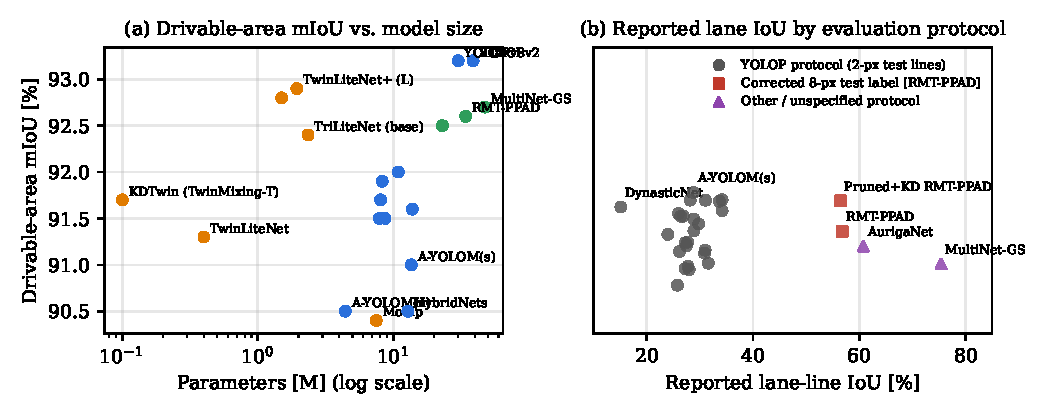
\includegraphics[width=0.98\linewidth]{figures/fig_tradeoff.pdf}
\caption{(a) Drivable-area mIoU versus parameter count as reported by the included studies (colours as in Fig.~\ref{fig:years}). (b) Reported lane IoU; the clusters correspond to different test-label protocols rather than to different model quality.}
\label{fig:tradeoff}
\end{figure}

\FloatBarrier
%=====================================================================
\section{Discussion}\label{sec:discussion}
%=====================================================================
\textbf{RQ1 -- approaches.} The field is dominated by hard parameter sharing on top of the current YOLO generation (Family A). Progress in this family mostly reflects progress in single-task detectors (CSPDarknet $\rightarrow$ ELAN $\rightarrow$ YOLOv8/GELAN), rather than new multi-task mechanisms. Explicit MTL techniques are rare and are usually reduced to fixed, hand-tuned loss weights. These techniques include uncertainty- or gradient-based loss balancing, task-conditioned feature routing, gating adapters~\cite{wang2026rmtppad} and adaptive concatenation~\cite{wang2024ayolom}. Only one study varies its loss balancing systematically~\cite{liang2023veprompt}, and one uses inter-task gradient conflict as a pruning criterion~\cite{compress2025}. The two newer trends are \emph{extreme miniaturisation} (Family B) and \emph{DETR-style query decoders} (Family C).

\textbf{RQ2 -- comparability.} The headline differences between consecutive methods (often $<1$\,pp in drivable mIoU, Table~\ref{tab:comparison}) are smaller than the differences created by protocol choices. Concrete sources of incomparability are: three or more meanings of ``lane accuracy''; two lane test-label widths; re-trained baselines with numbers that differ from the original papers; and internal inconsistencies. For example, YOLOP's drivable mIoU is quoted as 90.9, 91.1, 91.2 and 91.5 in different papers~\cite{ma2023grouped,liu2024gdmnet,mttppnet2025,wu2022yolop}. GDMNet reports two different detection results for the same model~\cite{liu2024gdmnet}, and MultiNet-GS lists YOLOP with 57.2\,M parameters instead of $\approx$7.9\,M~\cite{li2023multinetgs}. None of the 30 studies reports a standard deviation over seeds; one study explicitly notes that its results come from a single run~\cite{dbanet2026}. A ranking of methods by a fraction of a pp is therefore not statistically supported.

\textbf{RQ3 -- trade-offs.} Drivable-area segmentation is effectively solved at this resolution: models from 0.1 to 38.9\,M parameters all lie within 90--94\% mIoU (Fig.~\ref{fig:tradeoff}a). Model capacity pays off mainly for detection (recall 85--97\%, mAP@0.5 72--86\% under the standard protocol). Lightweight segmentation-only models are Pareto-optimal if detection is solved elsewhere. Embedded evaluation (Jetson, Atlas, mobile SoCs) is present in eight studies, but under heterogeneous conditions.

\textbf{RQ4 -- research gaps.} We identify four specific gaps.
\begin{enumerate}
\item \emph{No common evaluation protocol.} What is missing is an agreed, versioned evaluation script for the three-task BDD100K setting, with a fixed lane test label and explicitly defined metrics (IoU and balanced accuracy, or precision/recall/F1). Without it, a 0.3\,pp ``state-of-the-art'' claim cannot be distinguished from a protocol artefact (Fig.~\ref{fig:tradeoff}b). How to investigate: re-evaluate the released checkpoints of open-source methods (YOLOP, HybridNets, A-YOLOM, TwinLiteNet$^+$, TriLiteNet, RMT-PPAD) with one script, as RMT-PPAD started to do~\cite{wang2026rmtppad}, and publish a leaderboard with confidence intervals.
\item \emph{Statistical reliability.} No variance across seeds or bootstrap confidence intervals are reported. This matters because most improvements are within plausible run-to-run variation. How to investigate: at minimum, three training seeds per configuration and image-level bootstrap intervals on the 10k validation images.
\item \emph{Robustness and domain shift.} Most studies show night/rain only qualitatively; quantitative per-condition splits appear in three lightweight-model papers~\cite{che2025twinliteplus,trilitenet2025,twinmixing2026}, and cross-dataset evaluation is rare. This matters because BDD100K is US-centric and the only test bed, while~\cite{selvarajan2026safety} documents a clear domain gap for unstructured roads. How to investigate: report the BDD100K weather/time-of-day splits as standard and add zero-shot evaluation on a second dataset with compatible labels.
\item \emph{Comparable efficiency reporting and reproducibility.} Speed is measured on 12 GPUs with different protocols, and only 14 of 30 studies release code. How to investigate: report latency at batch size~1 with a fixed precision on one reference GPU and one embedded device, separating network time from pre- and post-processing, and release code and weights.
\end{enumerate}
In addition, the merged single-class vehicle detection inherited from YOLOP hides pedestrians, cyclists and traffic lights, which matter most for safety. Multi-class evaluation~\cite{liang2023veprompt} remains the exception.

%=====================================================================
\section{Replication Study}\label{sec:replication}
%=====================================================================
We replicated A-YOLOM~\cite{wang2024ayolom}, a Family~A model with a fully released implementation~\cite{ayolomcode}. It is representative of the dominant YOLOv8-based design, its pre-trained weights are public, and its authors define lane accuracy explicitly, which makes the metric verifiable.

\subsection{Experimental setup and procedure}
\textbf{What is replicated.} The evaluation results of Table~II--IV of~\cite{wang2024ayolom} (vehicle recall and mAP@0.5, drivable-area mIoU, lane balanced accuracy and IoU) for both released models, A-YOLOM(n) and A-YOLOM(s), on the full BDD100K validation set, together with the parameter count and inference speed of Table~I. Retraining (300 epochs on 3$\times$RTX~4090 in the original work) was out of scope for our hardware; we evaluate the authors' released checkpoints.

\textbf{Data.} The 10{,}000 validation images were taken from the official archive \texttt{bdd100k\_images\_100k.zip} (\url{http://dl.yf.io/bdd100k/}); our script fetches only the validation entries and verifies the CRC-32 of each file. We used the authors' converted annotations (detection, drivable area, lane) linked from the repository; they contain 70{,}000 training and 10{,}000 validation label files per task. \ReplDataNote

\textbf{Code and settings.} We used the official repository at commit \texttt{9cf56e8} without modifying any model or metric code. Our wrapper (\texttt{replication/eval\_ayolom.py}) calls the official \texttt{MultiValidator} with exactly the arguments of the repository's \texttt{val.py}: \texttt{imgsz=640}, \texttt{conf=0.001}, \texttt{iou=0.6}, \texttt{classes=[2,3,4,9,10,11]}, \texttt{combine\_class=[2,3,4,9]}, \texttt{single\_cls=True}, \texttt{batch=16}, and rectangular letterboxing (1280$\times$720 resized to 640$\times$360 and padded to a 672$\times$384 network input). As an addition, it accumulates a dataset-level confusion matrix per segmentation task. The official code averages the segmentation metrics \emph{per image}, and the dataset-level values show how much this choice matters.

\textbf{Device.} All accuracy numbers were computed on the \textbf{CPU}. Our first full run used the Apple GPU (MPS backend) and gave a much lower vehicle mAP@0.5 for A-YOLOM(n), 44.5\% instead of 78.0\%. We traced this to a backend defect rather than to the model (Section~\ref{sec:replres}). Speed was measured with \texttt{replication/fps\_benchmark.py}. It re-implements the authors' protocol: 5 warm-up passes, then 1000 forward passes of one 384$\times$640 input at batch size~1 and of the same input repeated 32 times. The original code path only supports CUDA, so we use the MPS synchronisation primitive instead. The network forward pass itself is numerically correct on MPS (maximum relative layer-wise difference to CPU $<3\cdot10^{-6}$).

\textbf{Environment.} \ReplEnvironment\ Random seed 0; the evaluation contains no stochastic component.

\textbf{Deviations from the original study.} (1)~Hardware: Apple M3~Pro (CPU for accuracy, MPS GPU for speed) instead of NVIDIA GPUs; FP32 throughout. (2)~Software: PyTorch~2.2.2 / Python~3.10 instead of PyTorch~1.13.1 / Python~3.7.16. (3)~No retraining; released weights only. (4)~Speed protocol re-implemented for MPS; absolute FPS is not comparable with the GTX~1080~Ti numbers of the paper.

\subsection{Results and discussion}\label{sec:replres}
\begin{table}[t]
\centering
\caption{Original versus replicated results of A-YOLOM on the BDD100K validation set (10{,}000 images). Original values: Tables~I--IV of~\cite{wang2024ayolom}. Replication: released weights, official evaluation code on the Apple M3~Pro CPU. Difference = replication $-$ original (pp for metrics). Parameters counted before Conv+BN fusion. $^\dagger$Original FPS on a GTX~1080~Ti, replication on Apple M3~Pro GPU (MPS, FP32) -- not comparable. $^\ddagger$Apple M3~Pro CPU, FP32, 100 passes.}
\label{tab:repl}
\small
\begin{tabular}{l rrr rrr}
\toprule
 & \multicolumn{3}{c}{A-YOLOM(n)} & \multicolumn{3}{c}{A-YOLOM(s)} \\
\cmidrule(lr){2-4}\cmidrule(lr){5-7}
Metric & Orig. & Repl. & Diff. & Orig. & Repl. & Diff. \\
\midrule
Vehicle recall [\%] & 85.3 & 85.27 & -0.03 & 86.9 & 86.90 & 0.00 \\
Vehicle mAP@0.5 [\%] & 78.0 & 78.00 & 0.00 & 81.1 & 81.08 & -0.02 \\
Drivable-area mIoU [\%] & 90.5 & 90.47 & -0.03 & 91.0 & 91.04 & +0.04 \\
Lane balanced accuracy [\%] & 81.3 & 81.33 & +0.03 & 84.9 & 84.88 & -0.02 \\
Lane IoU [\%] & 28.2 & 28.21 & +0.01 & 28.8 & 28.81 & +0.01 \\
\midrule
Parameters [M] & 4.43 & 3.64 & -0.79 & 13.61 & 13.61 & 0.00 \\
FPS, batch 1$^\dagger$ & 39.9 & 37.3 & n/a & 39.7 & 29.5 & n/a \\
FPS, batch 32$^\dagger$ & 172.2 & 101.2 & n/a & 96.2 & 53.5 & n/a \\
FPS, batch 1, CPU$^\ddagger$ & -- & 11.4 & n/a & -- & 6.1 & n/a \\
\bottomrule
\end{tabular}
\end{table}

\begin{table}[t]
\centering
\caption{Effect of the aggregation scheme on the segmentation metrics (replication, \%). The official code averages per-image values; ``dataset-level'' uses one confusion matrix accumulated over all 10{,}000 images.}
\label{tab:agg}
\small
\begin{tabular}{l rr rr}
\toprule
 & \multicolumn{2}{c}{A-YOLOM(n)} & \multicolumn{2}{c}{A-YOLOM(s)} \\
\cmidrule(lr){2-3}\cmidrule(lr){4-5}
Metric & per-image & dataset & per-image & dataset \\
\midrule
Drivable-area mIoU & 90.47 & 92.93 & 91.04 & 93.43 \\
Lane balanced accuracy & 81.33 & 84.01 & 84.88 & 87.68 \\
Lane IoU & 28.21 & 30.76 & 28.81 & 30.87 \\
\bottomrule
\end{tabular}
\end{table}

\begin{table}[t]
\centering
\caption{A-YOLOM(n): identical code, weights and data evaluated with the PyTorch~2.2.2 MPS (Apple GPU) backend versus the CPU (\%). We attribute the difference to in-place \texttt{clamp\_} operations on tensor views, which have no effect on MPS (see text).}
\label{tab:mps}
\small
\begin{tabular}{l rrr}
\toprule
Metric & CPU & MPS & Diff. \\
\midrule
Vehicle recall & 85.27 & 69.42 & -15.85 \\
Vehicle mAP@0.5 & 78.00 & 44.51 & -33.49 \\
Drivable-area mIoU & 90.47 & 90.20 & -0.27 \\
Lane balanced accuracy & 81.33 & 82.44 & +1.11 \\
Lane IoU (per-image) & 28.21 & 17.14 & -11.06 \\
Lane IoU (dataset-level) & 30.76 & 28.46 & -2.30 \\
\bottomrule
\end{tabular}
\end{table}


\ReplDiscussion

%=====================================================================
\section{Limitations}\label{sec:limitations}
%=====================================================================
\textbf{Search.} We used one Boolean query on three open indexes (OpenAlex, Semantic Scholar, arXiv) and did not query IEEE Xplore, Scopus or Web of Science directly. Papers that describe the task with other vocabulary (e.g.\ ``road segmentation'' without ``drivable area'') may have been missed; citation searching recovered two such baselines.
\textbf{Access bias.} The largest loss of evidence is at the retrieval stage. 60 of 91 eligible-looking records could not be read in full, mostly because they are behind paywalls (e.g.\ YOLOPX, Sparse U-PDP and MtpNet). The synthesis is therefore biased towards open-access venues (MDPI, arXiv, IEEE Access) and should be re-run with institutional access.
\textbf{Extraction and categorisation.} Values were extracted from text and tables as printed. Some publisher tables are images, which limited extraction for~\cite{liu2024fusion,mtfenet2025}. The assignment to three families is a judgement call, and extraction was LLM-assisted (Appendix~\ref{app:ai}). Publication bias towards positive ``state-of-the-art'' results is likely, as no negative results were found.
\textbf{Replication.} Without retraining, we verify the reported \emph{evaluation} of the released checkpoints, not the training procedure. Speed was measured on different hardware, and the evaluation uses the authors' converted labels rather than labels regenerated from the raw BDD100K JSON files.

%=====================================================================
\section{Conclusion}\label{sec:conclusion}
%=====================================================================
Between 2022 and 2026, multi-task panoptic driving perception has consolidated around YOLO-derived shared encoders, alongside a successful branch of sub-2\,M-parameter segmentation networks and an emerging branch of DETR-style query models (RQ1). All studies rely on BDD100K, but metric definitions (``lane accuracy''), lane test labels, re-trained baselines and speed protocols differ so much that the frequently claimed sub-point improvements are not comparable (RQ2). Drivable-area segmentation has saturated around 92--94\% mIoU regardless of model size, while detection still benefits from capacity (RQ3). The most important open problems are a common, versioned evaluation protocol, statistical reporting over repeated runs, quantitative robustness and cross-dataset evaluation, and comparable efficiency reporting with released code (RQ4). \ReplConclusion\ (RQ5).

\appendices
\section{Use of generative AI / LLM}\label{app:ai}
\textbf{Tool and model.} Claude Code (desktop application, Anthropic) with the model Claude Opus~5.5 (\texttt{claude-opus-5-5}), used on 25~November~2026.

\textbf{Purpose of use.}
(1)~Writing and running the search scripts for OpenAlex, Semantic Scholar and arXiv, and de-duplicating the records;
(2)~proposing title/abstract screening decisions (all decisions and reasons are listed in \path{review/search/screening.csv});
(3)~reading open-access full texts and extracting the data items of Section~\ref{sec:method}. Sub-agents of the same model read arXiv/HTML versions; other values were read by the assistant from publisher HTML tables in a browser or from PDF text extracted with \texttt{pypdf};
(4)~fetching bibliographic metadata from Crossref/arXiv to build the reference list;
(5)~setting up the software environment, writing the evaluation, data-download and speed-benchmark scripts, running the replication and generating the tables and figures;
(6)~drafting the text of this article.
The LLM is not a scientific source. Every number in Tables~\ref{tab:qual}--\ref{tab:comparison} must be traceable to the primary source listed in the extraction table (\path{review/included_studies.csv}), and the authors are responsible for checking it. Values that the assistant could not verify from the full text were recorded as ``not reported'' rather than estimated.

\textbf{Prompts.} The task-level prompt given by the authors (verbatim, except that diacritics in the attached file name were removed for typesetting):
\begin{lstlisting}
@"Systematicky prehlad literatury_replikacia experimentu (1).pdf"
https://github.com/JiayuanWang-JW/YOLOv8-multi-task.git
i want you to use this github. I need it for the .pdf
So go to work. No mistakes.
\end{lstlisting}
Clarifying answers given by the authors when asked by the assistant: download of the weights, annotations and BDD100K images approved; article language English; replication scope ``evaluation only''; author names left as placeholders. The only further prompt by the authors was a status question during the run (verbatim):
\begin{lstlisting}
how long until it's done?
\end{lstlisting}

Data-extraction prompt sent to the reading sub-agents (abridged only by removing the per-paper URL list):
\begin{lstlisting}
You are doing data extraction for a systematic literature review on camera-based multi-task
"panoptic driving perception" (traffic object detection + drivable area segmentation + lane
line detection/segmentation, mainly on BDD100K). Read the FULL TEXT (not just the abstract) of
each paper below at the given URL. Report ONLY what the paper itself states. Never guess or
fill from memory; if a value is not stated write "NR". Copy numbers exactly as printed (keep
the paper's precision and units). For numbers, say which table they come from.
For EACH paper return one JSON object with these keys: "rid", "title", "venue_year_as_printed",
"full_text_read", "tasks_evaluated", "datasets", "input_resolution", "method_summary",
"det_classes", "own_results_bdd100k": {"det_recall","det_mAP50","det_mAP50_95","da_mIoU",
"ll_acc","ll_IoU","params","gflops","fps","fps_hardware_and_batch"}, "lane_acc_definition",
"baselines_compared", "robustness_or_extra_eval", "code_available",
"limitations_stated_by_authors", "exclusion_flag".
\end{lstlisting}


\bibliographystyle{IEEEtran}
\bibliography{refs}

\end{document}
